\begin{figure*}[!hbt]
  \centering
  \subfigure[Overall Runtime]{
    \label{fig:temporal-summary--runtime-overall}
    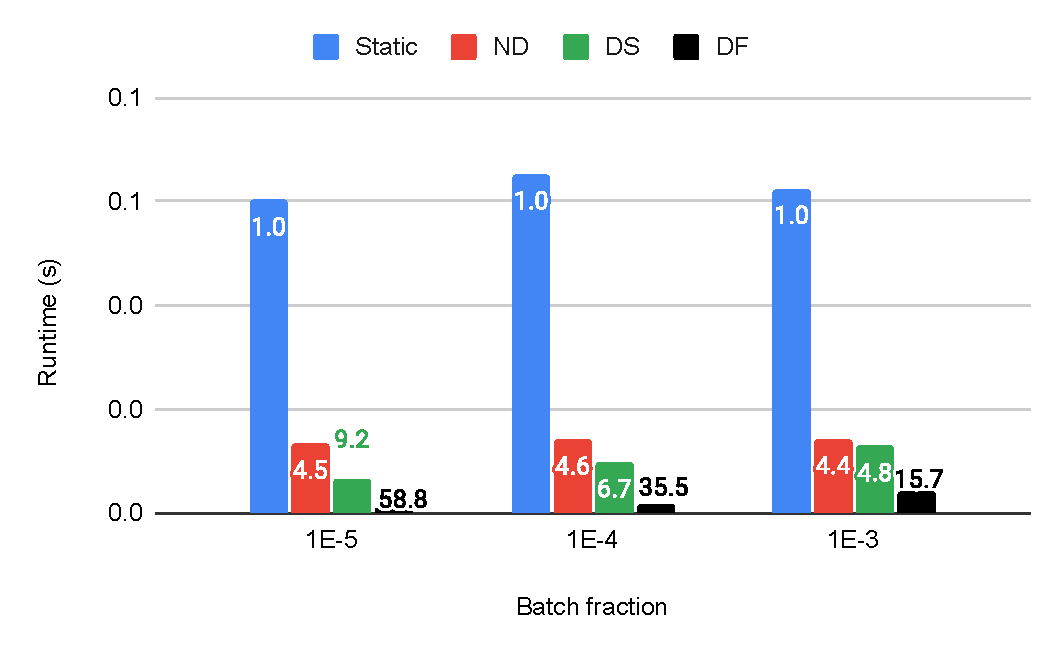
\includegraphics[width=0.48\linewidth]{out/temporal-summary-runtime-overall.pdf}
  }
  \subfigure[Overall Modularity of communities obtained]{
    \label{fig:temporal-summary--modularity-overall}
    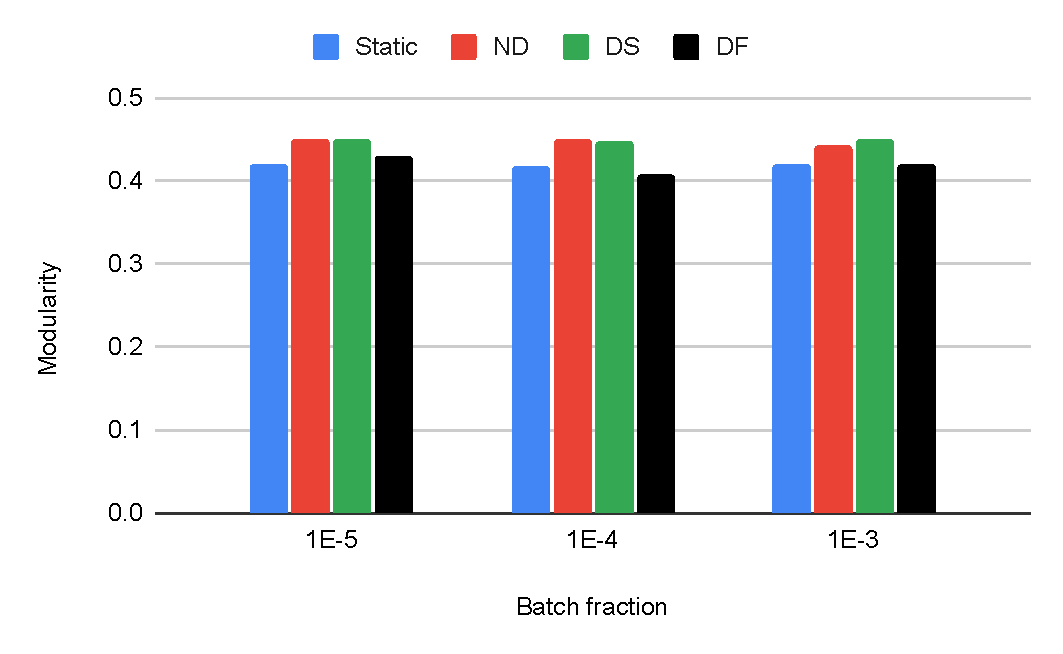
\includegraphics[width=0.48\linewidth]{out/temporal-summary-modularity-overall.pdf}
  } \\[2ex]
  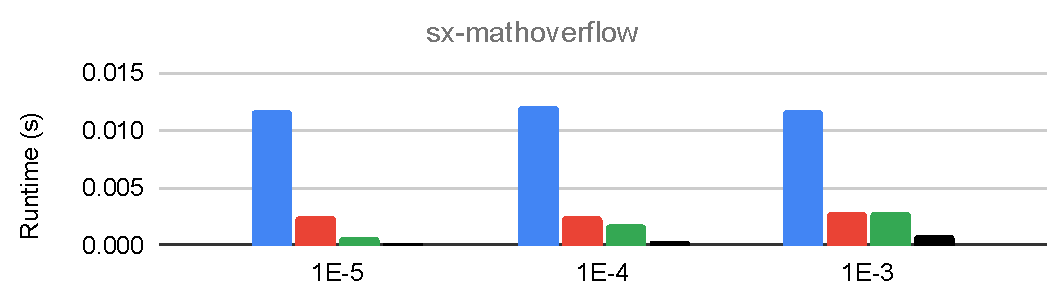
\includegraphics[width=0.48\linewidth]{out/temporal-summary-runtime-sx-mathoverflow.pdf}
  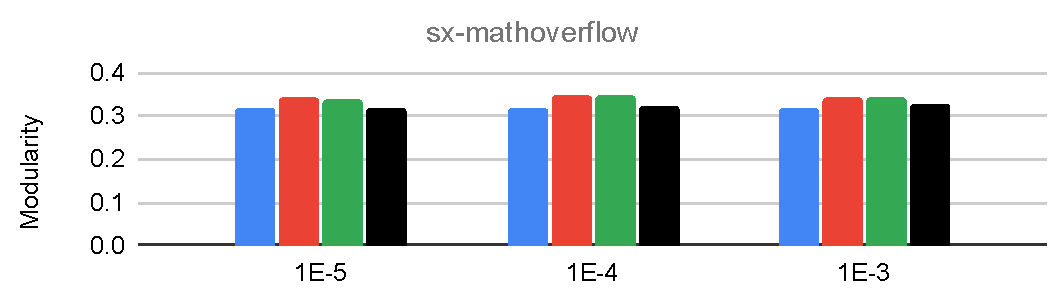
\includegraphics[width=0.48\linewidth]{out/temporal-summary-modularity-sx-mathoverflow.pdf}
  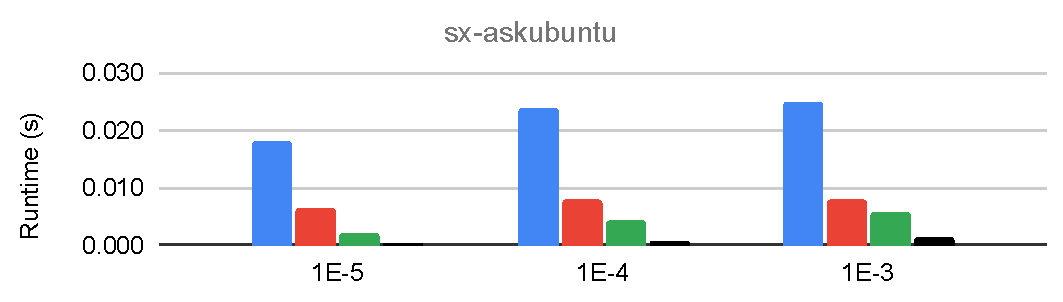
\includegraphics[width=0.48\linewidth]{out/temporal-summary-runtime-sx-askubuntu.pdf}
  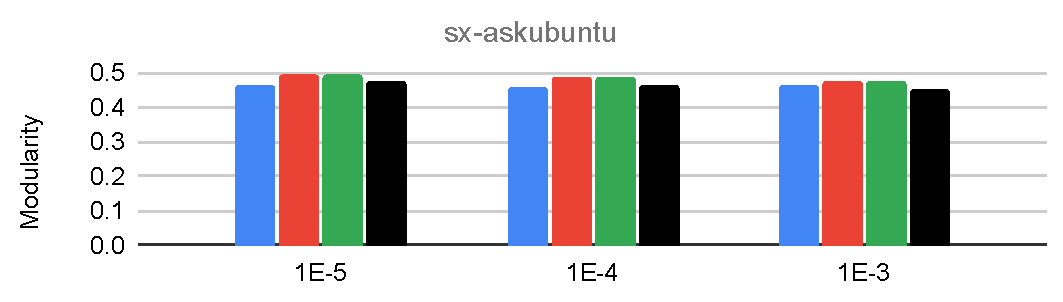
\includegraphics[width=0.48\linewidth]{out/temporal-summary-modularity-sx-askubuntu.pdf}
  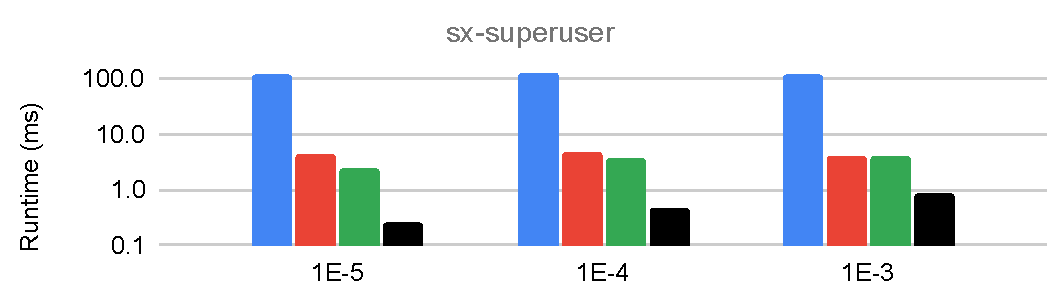
\includegraphics[width=0.48\linewidth]{out/temporal-summary-runtime-sx-superuser.pdf}
  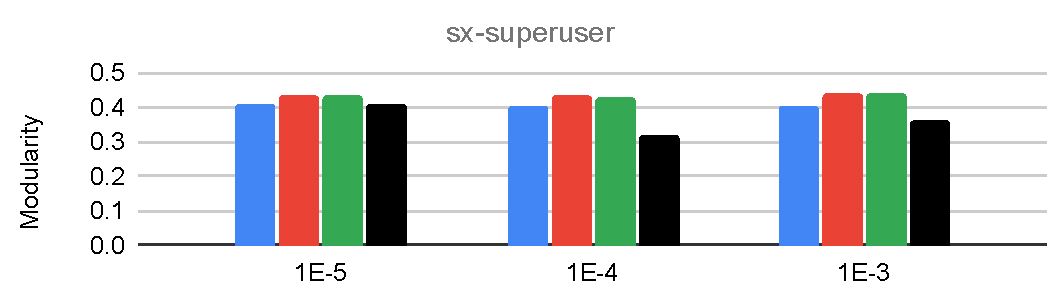
\includegraphics[width=0.48\linewidth]{out/temporal-summary-modularity-sx-superuser.pdf}
  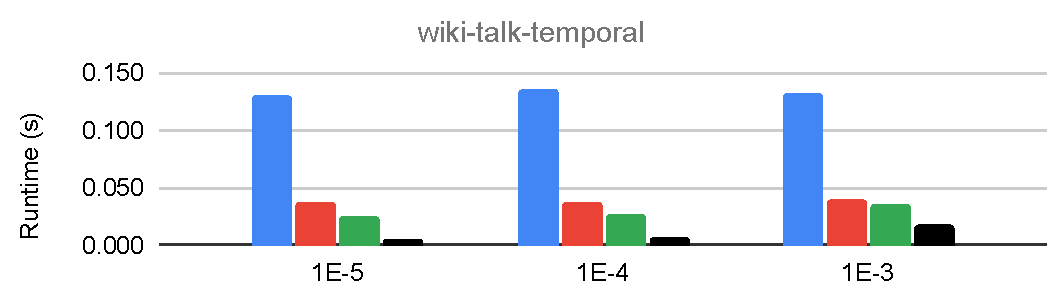
\includegraphics[width=0.48\linewidth]{out/temporal-summary-runtime-wiki-talk-temporal.pdf}
  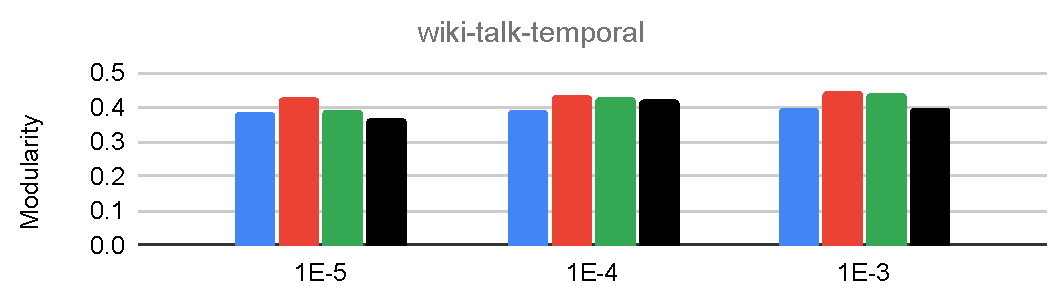
\includegraphics[width=0.48\linewidth]{out/temporal-summary-modularity-wiki-talk-temporal.pdf}
  \subfigure[Runtime on each dynamic graph]{
    \label{fig:temporal-summary--runtime-graph}
    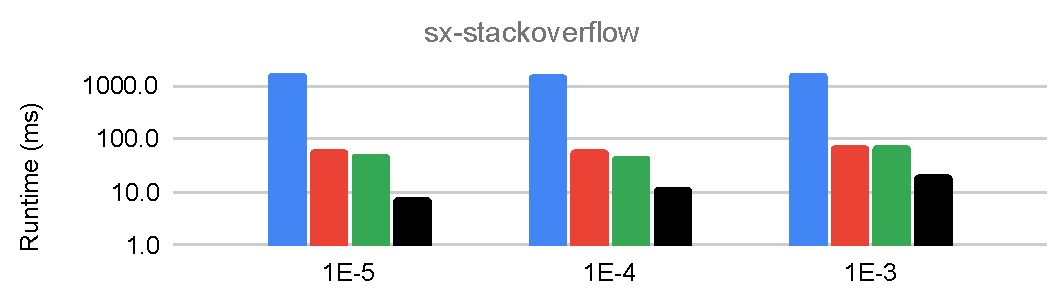
\includegraphics[width=0.48\linewidth]{out/temporal-summary-runtime-sx-stackoverflow.pdf}
  }
  \subfigure[Modularity in communities obtained on each dynamic graph]{
    \label{fig:temporal-summary--modularity-graph}
    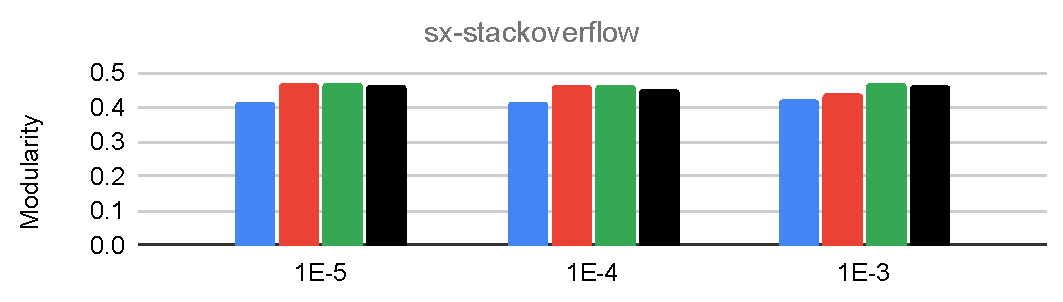
\includegraphics[width=0.48\linewidth]{out/temporal-summary-modularity-sx-stackoverflow.pdf}
  } \\[-2ex]
  \caption{Mean Runtime and Modularity of communities obtained with our GPU implementation of \textit{Static}, \textit{Naive-dynamic (ND)}, \textit{Dynamic Traversal (DT)}, \textit{Dynamic Frontier (DF)}, and \textit{Dynamic Frontier with Pruning (DF-P)} PageRank on real-world dynamic graphs, with batch updates of size $10^{-5}|E_T|$ to $10^{-3}|E_T|$. Here, (a) and (b) show the overall runtime and modularity across all temporal graphs, while (c) and (d) show the runtime and rank modularity for each approach (relative to reference Static PageRank, see Section \ref{sec:measurement}). In (a), the speedup of each approach with respect to Static PageRank is labeled.}
  \label{fig:temporal-summary}
\end{figure*}
